\documentclass{article}%
\usepackage[T1]{fontenc}%
\usepackage[utf8]{inputenc}%
\usepackage{lmodern}%
\usepackage{textcomp}%
\usepackage{lastpage}%
\usepackage[head=40pt,margin=0.5in,bottom=0.6in]{geometry}%
\usepackage{graphicx}%
%
\title{\textbf{Acnur pidió más "coherencia regional" ante el éxodo de venezolanos}}%
\author{EFE}%
\date{01/10/2018}%
%
\begin{document}%
\normalsize%
\maketitle%
\textbf{URL: }%
http://www.eluniversal.com/politica/22015/acnur{-}pide{-}mas{-}coherencia{-}regional{-}ante{-}el{-}exodo{-}de{-}venezolanos\newline%
%
\textbf{Periodico: }%
EU, %
ID: %
22015, %
Seccion: %
politica\newline%
%
\textbf{Palabras Claves: }%
NO\_TIENE\newline%
%
\textbf{Derecho: }%
CONTEXTO, %
Otros Derechos: %
, %
Sub Derechos: %
\newline%
%
\textbf{EP: }%
NO\newline%
\newline%
%
\textbf{\textit{Quito albergó en septiembre un encuentro en que se analizó por primera vez desde un enfoque regional los distintos escenarios que plantea el fenómeno del éxodo de venezolanos a sus países vecinos}}%
\newline%
\newline%
%
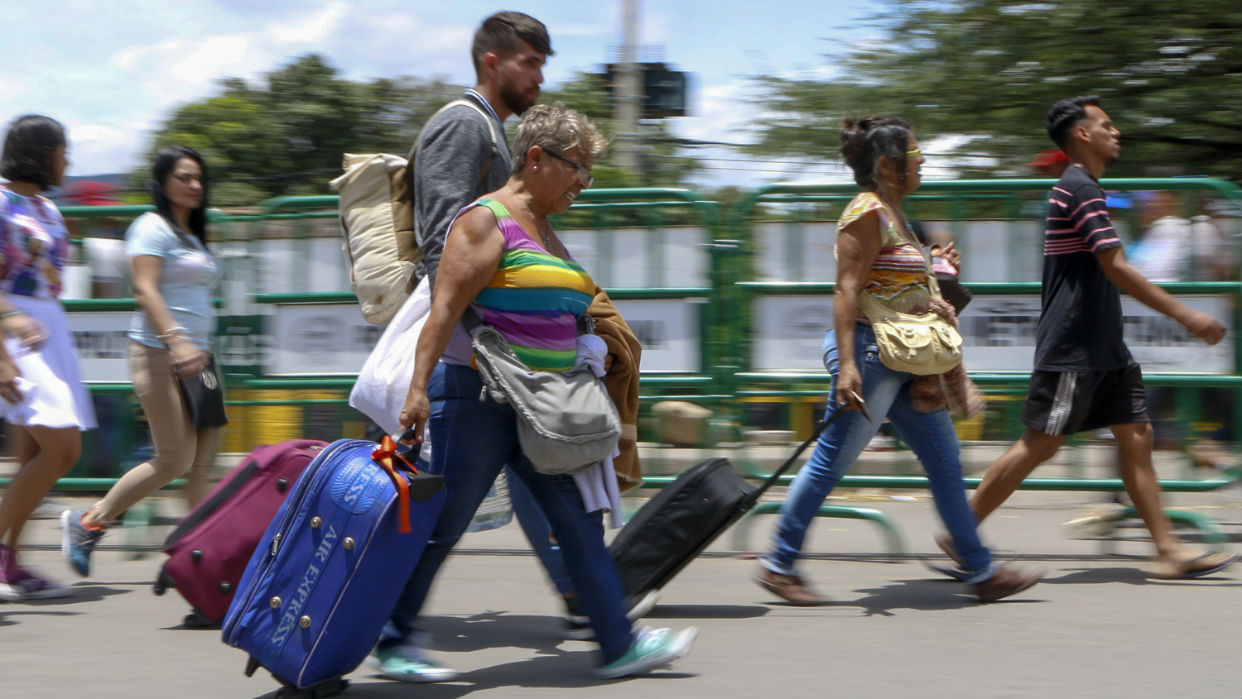
\includegraphics[width=300px]{183.jpg}%
\newline%
%
Ginebra.{-} El alto comisionado de Naciones Unidas para los Refugiados, Filippo Grandi, felicitó este lunes a los países latinoamericanos firmantes de la Declaración de Quito, pero les pidió más "coherencia regional" en su respuesta al éxodo venezolano.%
\newline%
%
"Aplaudo la respuesta regional adoptada en la Declaración de Quito y alabo a los estados de la región por mantener sus fronteras abiertas y permitir el acceso al asilo y otras alternativas legales para la estancia", afirmó Grandi en su discurso de inauguración del Comité Ejecutivo del organismo, que comenzó hoy en Ginebra.~"Sin embargo {-}agregó{-} se necesita más coherencia regional en la respuesta de protección".%
\newline%
%
Grandi asumió que los países necesitan "apoyo" y por ello recordó que Acnur junto a la Organización Internacional de las Migraciones (OIM) ha establecido una plataforma de coordinación regional y han designado un representante especial, Eduardo Stein, para que trabaje con los gobiernos para crear alianzas regionales y ayudar a los países receptores.%
\newline%
%
Quito albergó en septiembre un encuentro en que se analizó por primera vez desde un enfoque regional los distintos escenarios que plantea el fenómeno del éxodo de venezolanos a sus vecinos latinoamericanos, reseñó Efe.%
\newline%
%
El encuentro concluyó con una declaración rubricada por once de los países asistentes con la que se comprometieron a de redoblar los esfuerzos y flexibilizar las medidas exigidas a los migrantes, así como la necesidad de buscar soluciones a medio plazo puesto que muchos de los que emigran llegan a los países para quedarse.%
\newline%
%
De acuerdo a cifras recabadas por Acnur y la OIM cerca de 2,5 millones de personas han salido de Venezuela desde 2014.%
\newline%
%
\end{document}